\documentclass{beamer}
\usepackage{transparent}
\usepackage[beamer]{shortcut}


\usepackage{animate}
\usepackage{bibentry}
\usepackage{appendixnumberbeamer}

\graphicspath{{../thesis/figures/},{./images/}}
\def\TikzLocation{./tikz/}
\def\tkzscl{1}

\def\onecol{}
\def\twocols{}
\def\twoblocks{}
% \def\btitle{}
\def\bimplies{}
\def\partintro{}


\definecolor{primary}{RGB}{191,213,219}
\definecolor{secondary}{RGB}{144,106,66}
\setbeamercolor{block title}{fg=darkred}
\newcommand{\btitle}[1]{{\usebeamerfont{block title}\usebeamercolor[fg]{block title} #1}}


\setbeamertemplate{frametitle}{
  \begin{beamercolorbox}[left, leftskip=1ex,colsep*=.5em,wd=\paperwidth]{block title}
	\usebeamerfont*{frametitle}{\phantom{Gg}\hskip-3ex\insertframetitle}
  \end{beamercolorbox}
  \vskip-1em
  \begin{beamercolorbox}[wd=\paperwidth]{separation line}
    \rule{0pt}{1pt}
  \end{beamercolorbox}
}

\AtBeginSection[]
{
}


\makeatletter
\def\beamer@newblock{%
  \usebeamercolor[fg]{bibliography entry author}%
  \usebeamerfont{bibliography entry author}%
  \usebeamertemplate{bibliography entry author}%
  \def\newblock{%
    \usebeamercolor[fg]{bibliography entry title}%
    \usebeamerfont{bibliography entry title}%
    \usebeamertemplate{bibliography entry title}%
    \def\newblock{%
      \usebeamercolor[fg]{bibliography entry location}%
      \usebeamerfont{bibliography entry location}%
      \usebeamertemplate{bibliography entry location}%
      \def\newblock{%
        \usebeamercolor[fg]{bibliography entry note}%
        \usebeamerfont{bibliography entry note}%
        \usebeamertemplate{bibliography entry note}}}}%
  \leavevmode\setbox\beamer@tempbox=\hbox{}\ht\beamer@tempbox=0em\box\beamer@tempbox}
  \setbeamertemplate{bibliography entry title}{}{}

\makeatother

\usepackage[square, authoryear]{natbib}


%-----------------------------------------------------------------------------
%	CUSTOM COMANDS
%-----------------------------------------------------------------------------

\def\keypoint#1{\hfill\textcolor{gray}{#1}}
\def\mycite#1{\keypoint{\citep{#1}}}
\def\biblio{
	\nobibliography{../../library}
	\def\biblio{}
}




%\usepackage{lxfonts}

\institute{Ph.D. Defense ~--~ École Normale Supérieure Paris-Saclay}
\author{Thomas Moreau}
\title{Représentations Convolutives}

\date{
  Dec. 19, 2017\\[2.5ex]
  \hspace{3ex}Committee:\\[1ex]
  \noindent
  \begin{tabular}{@{}lp{7em}ll}
    Stéphanie Allassonière & Examiner &
    Alexandre Gramfort & Examiner\\
    Pierre-Paul Vidal & Examiner &
    René Vidal & Referee\\
    Stéphane Mallat & Referee &
    Julien Mairal & Referee\\
    Nicolas Vayatis & Supervisor &
    Laurent Oudre & Co-supervisor
  \end{tabular}
}

\setbeamertemplate{title page}[frame]


\begin{document}

\begin{frame}[plain]
\titlepage
\biblio{}
\end{frame}


\subfile{motiv}

%========================================================================
\section{Accelerating Convolutional\\Sparse Coding: DICOD}
%========================================================================


\begin{frame}[t]
  \vskip5em
  \centering
  \begin{beamercolorbox}[sep=8pt,center,shadow=true,rounded=true]{title}
    \usebeamerfont{title}\insertsectionhead%
  \end{beamercolorbox}
  \vskip5em
  \flushleft
	\textbf{References}
		\small\vskip.5em
		\bibentry{Moreau2015}\\[.5em]
		\bibentry{Moreau2017a}
\end{frame}

\subfile{dicod}


%========================================================================
\section{Adaptive Sparse Coding}
%========================================================================
\begin{frame}[t]
  \vskip5em
  \centering
  \begin{beamercolorbox}[sep=8pt,center,shadow=true,rounded=true]{title}
    \usebeamerfont{title}\insertsectionhead%
  \end{beamercolorbox}
  \vskip5em
  \flushleft
	\textbf{References}
		\small\vskip.5em
		\bibentry{Moreau2017}
\end{frame}

\subfile{lista}


%===========================================================================
\section{Conclusion}
%===========================================================================

\begin{frame}[noframenumbering,plain,t]
  \vskip8em
  \begin{center}
    \Huge
    Thanks!    
  \end{center}
  \vskip8em
  \vfill
  \begin{itemize}
			\item Co-authors: L. Oudre, N. Vayatis, J. Bruna.
			\item Medical doctors: S. Buffat, D. Ricard, M. Robert, P-P. Vidal, C. de Waele, A. Yelnik, R. Barrois.
		\end{itemize}
\end{frame}

%===========================================================================
% AUXILIARY SLIDES
%===========================================================================



%===========================================================================
\appendix
\section{Auxiliary Slides}
%===========================================================================


%===========================================================================
\subsection{Physiological Signals}
%===========================================================================


\begin{frame}{Experiment}
		Create a dictionary with 25 Gaussian patterns ($W=90$)
		\[
			\pmb D^{(0)}_k \sim \mathcal N(0, I_{90})
		\]
		\vskip1em
		Use the Convolutional Dictionary Learning with\\
		DICOD to learn a dictionary $\pmb D$ on a set of $50$\\
		recording of healthy subjects walking.
		\vskip2em
		\btitle{Challenges}
		\vskip.5em
		\begin{itemize}\itemsep.5em
			\item Alignment of the patterns,
			\item Detect steps of different amplitude,
			\item Handle multivariate signals.
		\end{itemize}

\end{frame}
\begin{frame}{Experiment}
		\centering
		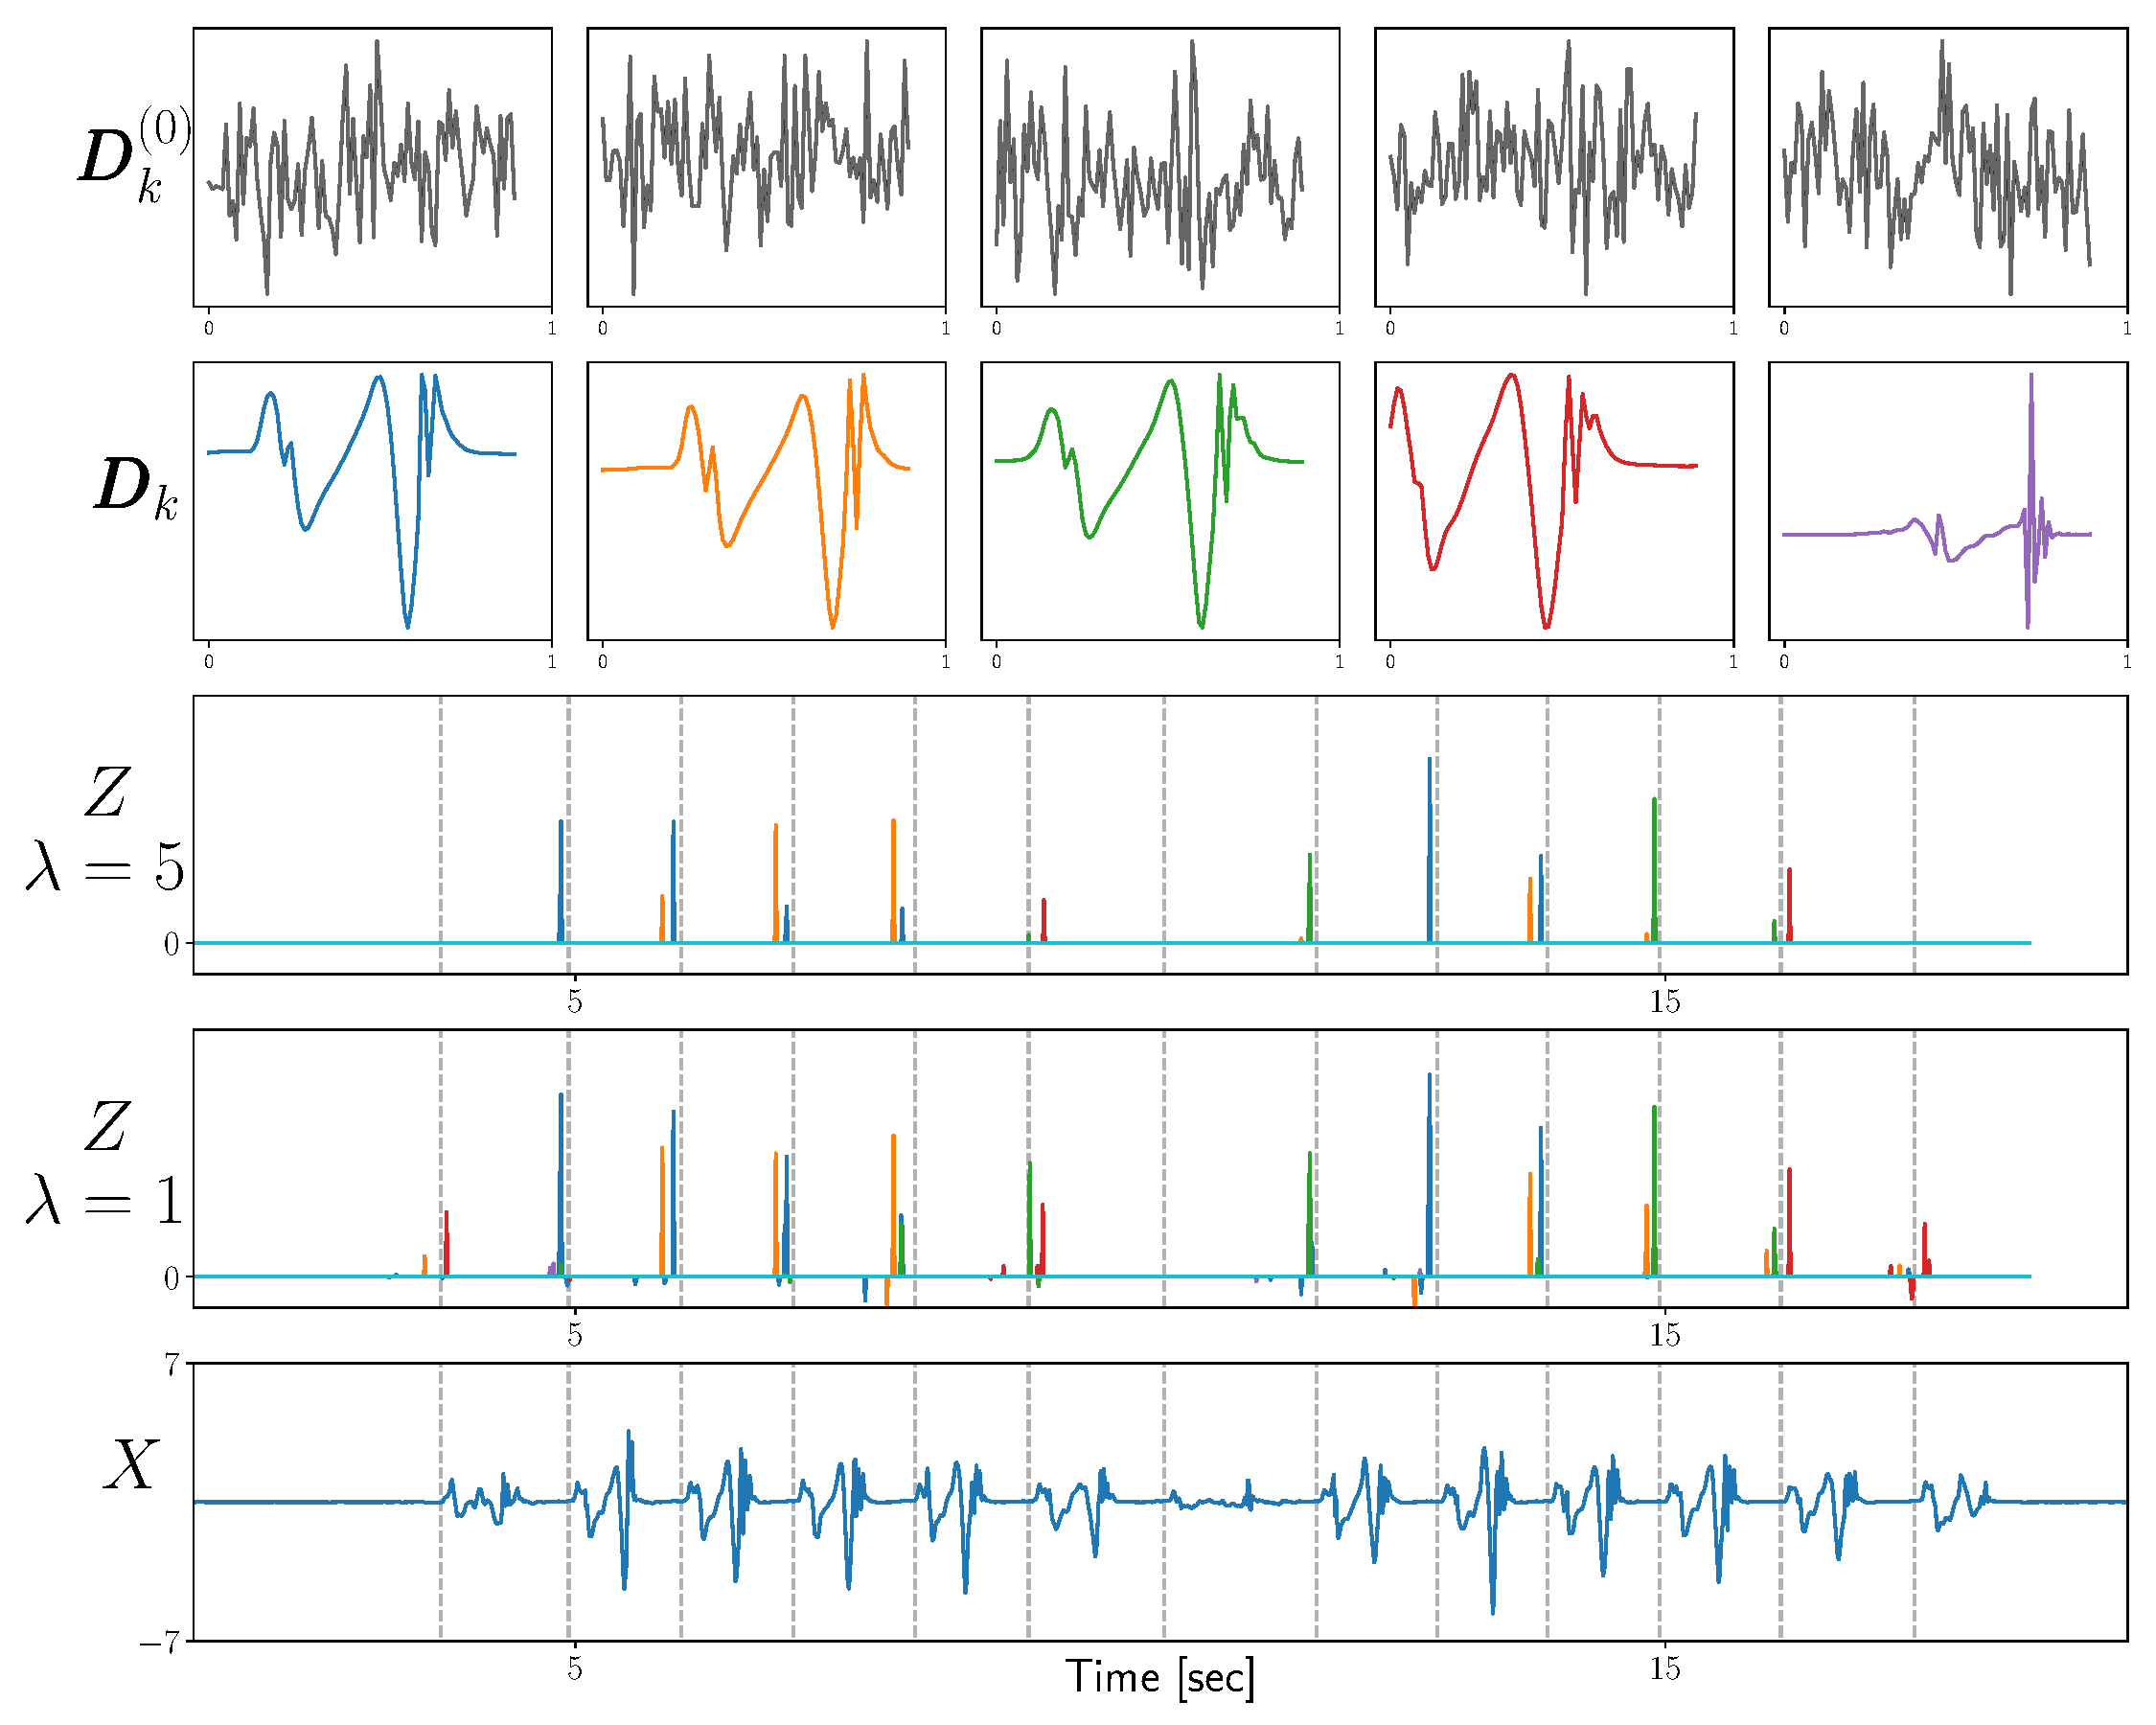
\includegraphics[width=.8\textwidth]{csc_random_defense}

\end{frame}

\begin{frame}
	\begin{block}{Publications and preprints}
		\tiny\vskip.5em
		\bibentry{Moreau2015a}\\[.5em]
		\bibentry{Oudre2015}\\[.5em]
		\bibentry{Moreau2015}\\[.5em]
		\bibentry{Moreau2016}\\[.5em]
		\bibentry{Moreau2017}\\[.5em]
		\bibentry{Moreau2017a}\\[.5em]
		\bibentry{Barrois2015}\\[.5em]
		\bibentry{Barrois2016}\\[.5em]
		\bibentry{Robert2015}\\[.5em]
    \end{block}
\end{frame}



\begin{frame}
\twocols{


}{
	\centering
	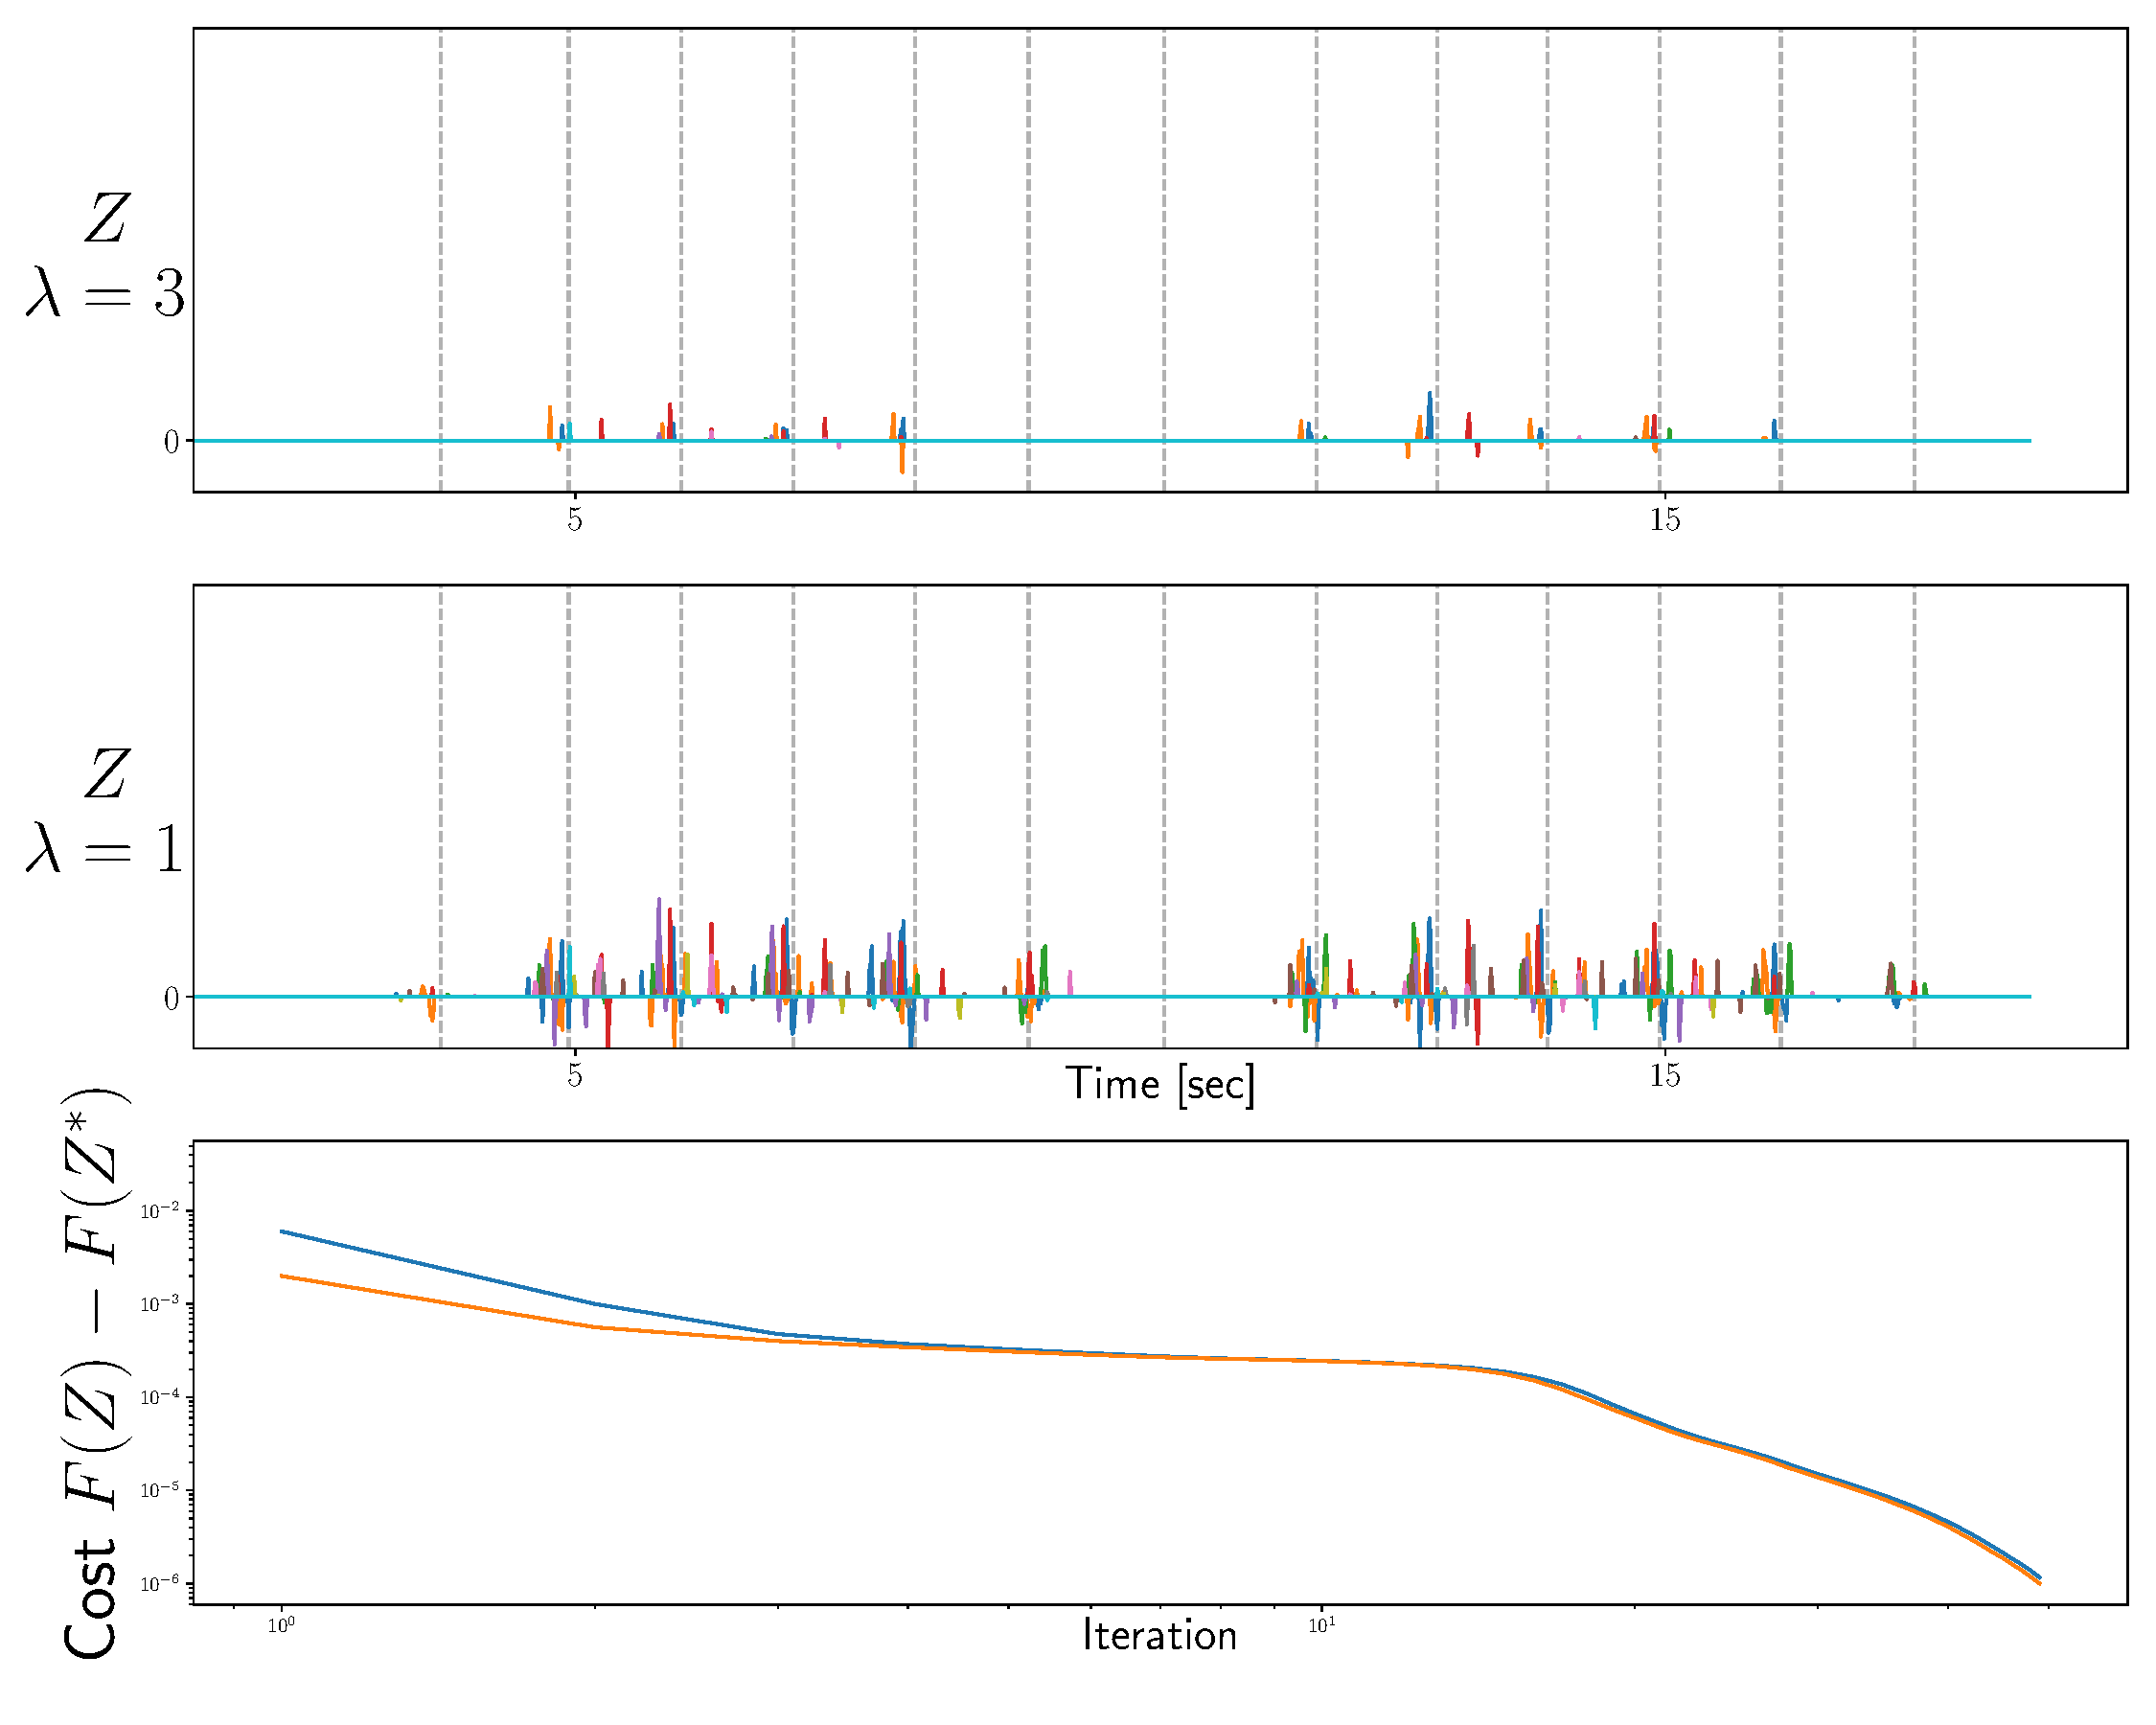
\includegraphics[width=\textwidth]{csc_random_annex}
}
	
\end{frame}

%===========================================================================
\subsection{FacNet}
%===========================================================================


\begin{frame}{Related works}

\twoblocks{}{
\begin{itemize}\itemsep2em
	\item \cite{Giryes2016}: Propose the inexact projected gradient descent and conjecture that LISTA accelerate the LASSO resolution by learning the sparsity pattern of the input distribution.
	\item \cite{xin2016maximal}: Study the Hard-thresholding Algorithm and its
	capacity to recover the support of a sparse vector.\\
	The paper relax the RIP conditions for the dictionary.
\end{itemize}
}{}{}
\end{frame}


\begin{frame}
	
	\twoblocks{Generic Dictionaries}{
	\vskip2em
	A dictionary $D \in \Rset^{p\times K}$ is a generic dictionary when its columns
	$D_i$ are drawn uniformly over the $\ell_2$ unit sphere $\mathcal S^{p-1}$.

	}{Theorem (Generic Acceleration)}{
	\vskip1em
	In \textbf{expectation over the generic dictionary} $D$, the factorization algorithm using a
		diagonally dominant matrix $A\subset\mathcal E_\delta$, has better performance for
		iteration $q+1$ than the normal ISTA iteration -- which uses the identity -- when
		\[
			\lambda\E[z]{\|z^{(q+1)}\|_1+\|z^*\|_1}
				\le \sqrt{\frac{K(K-1)}{p}} \underbrace{\E[z]{\|z^{(q)}-z^*\|_2^2}
				}_{\substack{\text{expected resolution}\\\text{at iteration $q$ }}}
		\]

	\vskip2em
	FacNet can improve the performances compared to ISTA when this is verified.}
\end{frame}



\begin{frame}
\twoblocks{L-FISTA}{
	\centering
	\vskip4em
	\inputTikZ{.65}{lifsta_tikz}
	\vskip2em
	Network architecture for L-FISTA.
}{}{
	\centering
	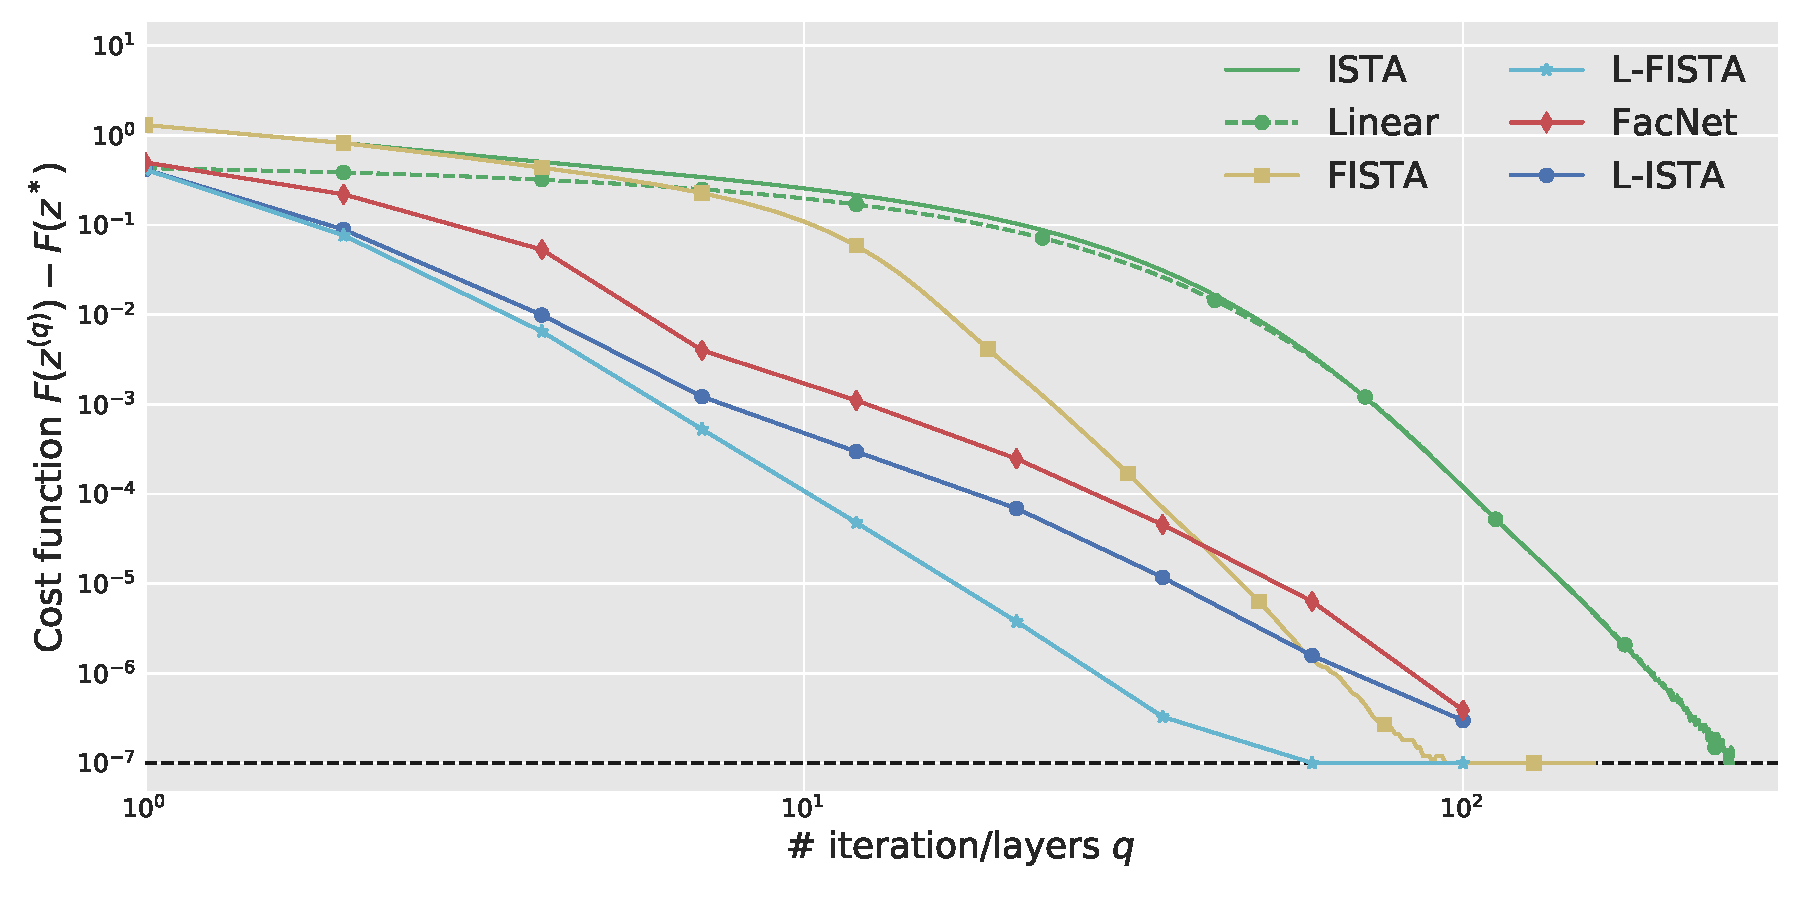
\includegraphics[width=\textwidth]{curve_sparse005_seaborn}
    Evolution of the cost function $F(z^{(q)}) - F(z^*)$ with the number
   	of layers/iterations $q$ with a denser model
}
	
\end{frame}
\begin{frame}

	\twocols{
		\centering
		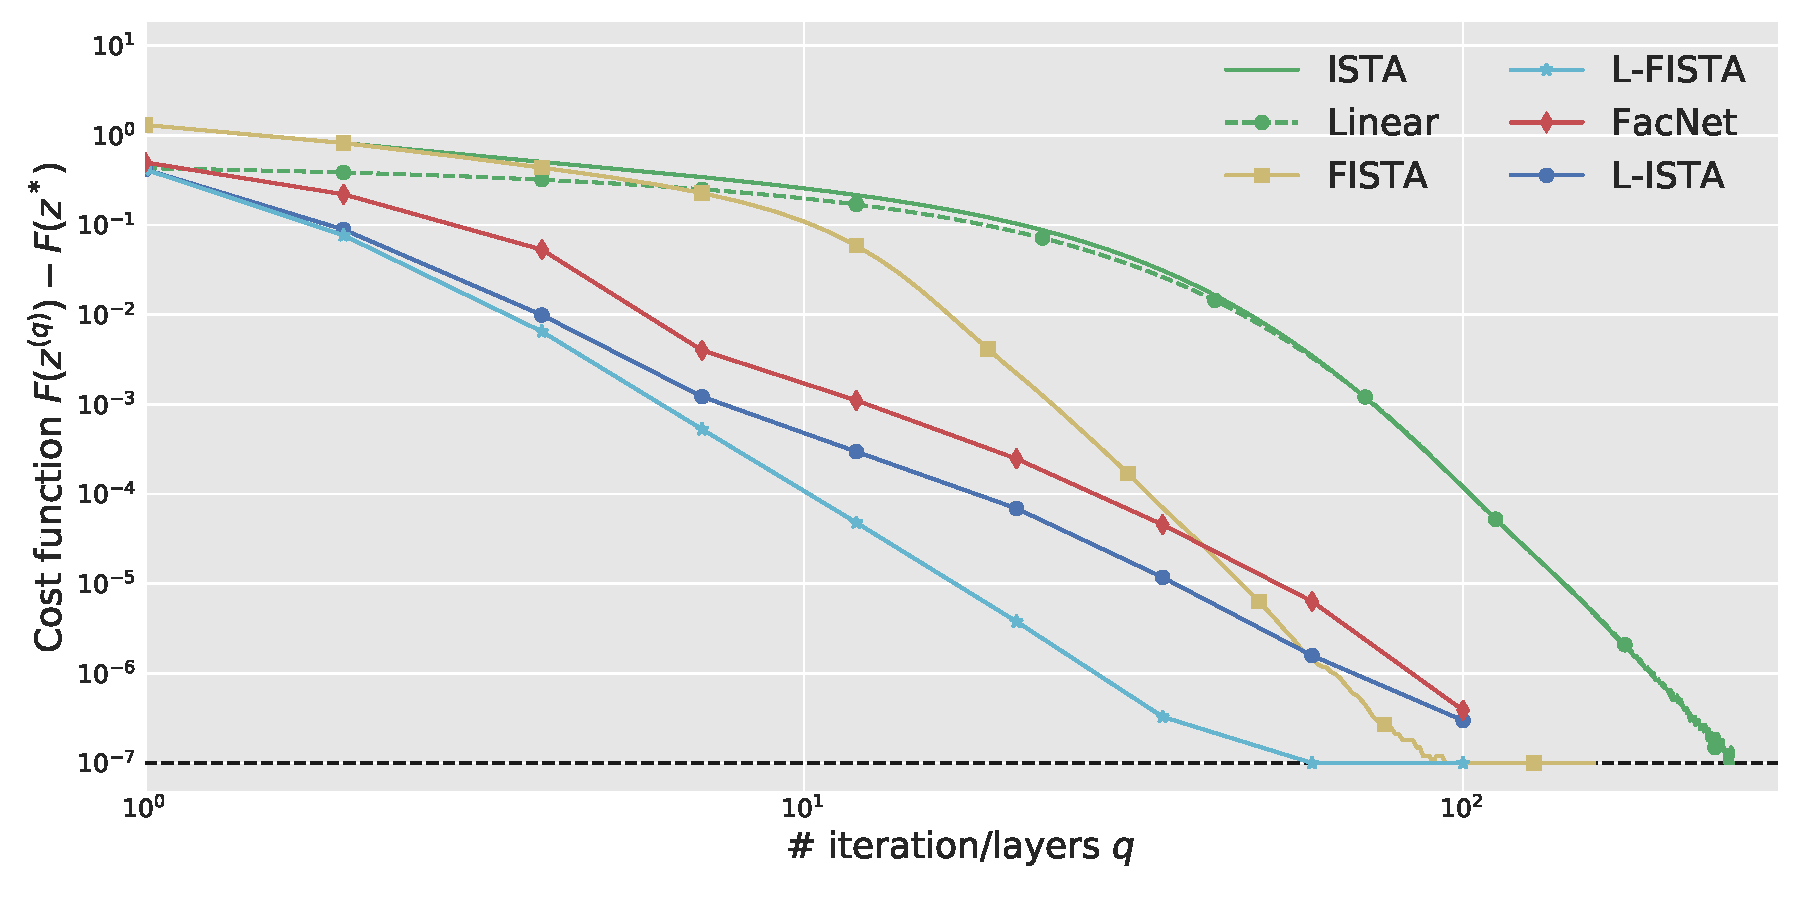
\includegraphics[width=\textwidth]{curve_sparse005_seaborn}\\
		$\rho = {}^1/_{20}$.\\[1em]

		Evolution of the cost function $F(z^{(q)}) - F(z^*)$ with the number
	   	of layers/iterations $q$ with a denser model

	}{
		\centering
		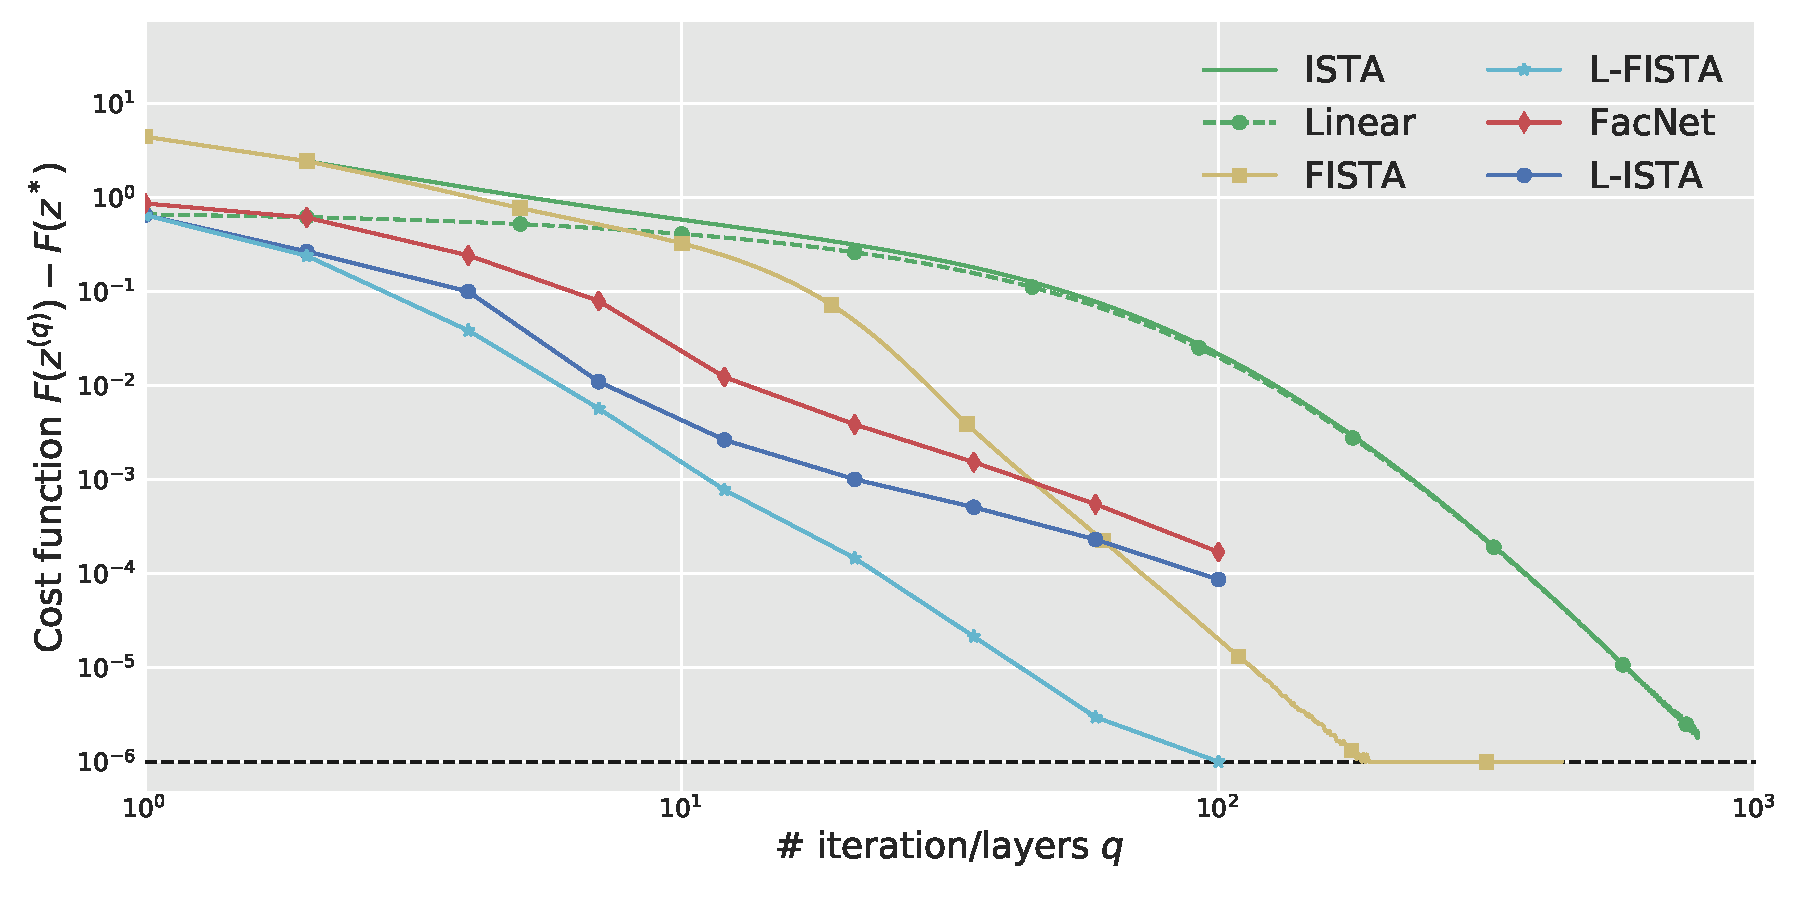
\includegraphics[width=\textwidth]{curve_sparse02_seaborn}\\
		$\rho = {}^1/_{4}$.\\[1em]
		Evolution of the cost function $F(z^{(q)}) - F(z^*)$ with the number
	   	of layers/iterations $q$ with a denser model
	}
\end{frame}


\begin{frame}{PASCAL 08}
\twocols{
	\btitle{PASCAL 08}
	\vskip1em
	Sparse coding for the PASCAL 08 datasets over the Haar wavelets family.\\[1em]
	\emph{Patch size:} 8x8;~~~$K = 267$;~~~  \emph{train/test:} 500/100\\[1em]
	\centering
	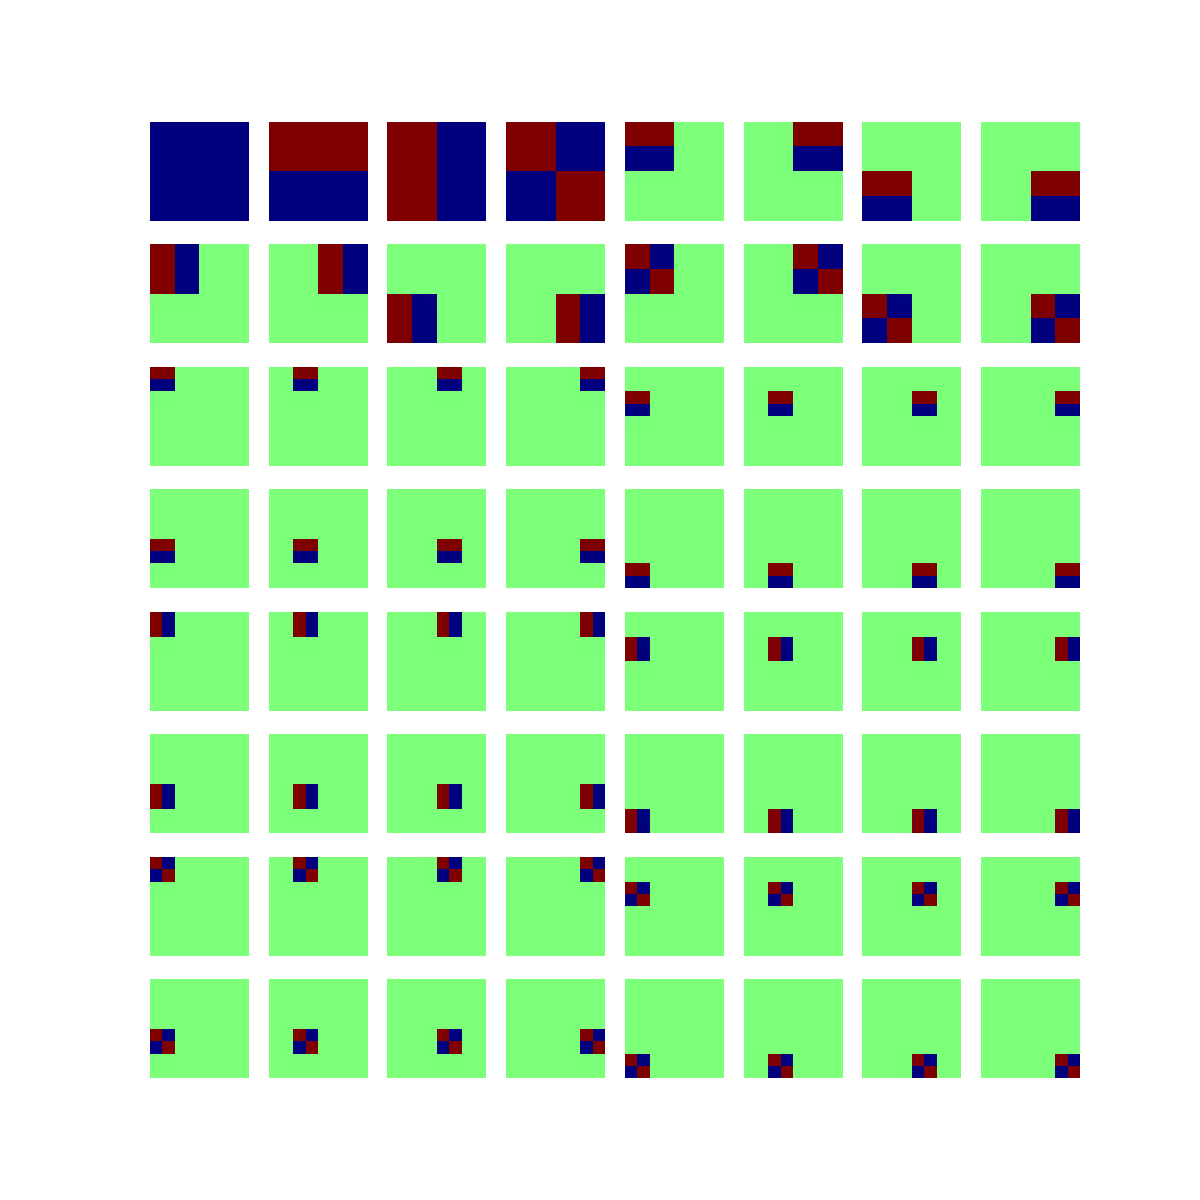
\includegraphics[width=.6\textwidth, trim={5em 4em 4em 4em}, clip]{Wavelets}\\
}{
	\vskip5em
    \centering
    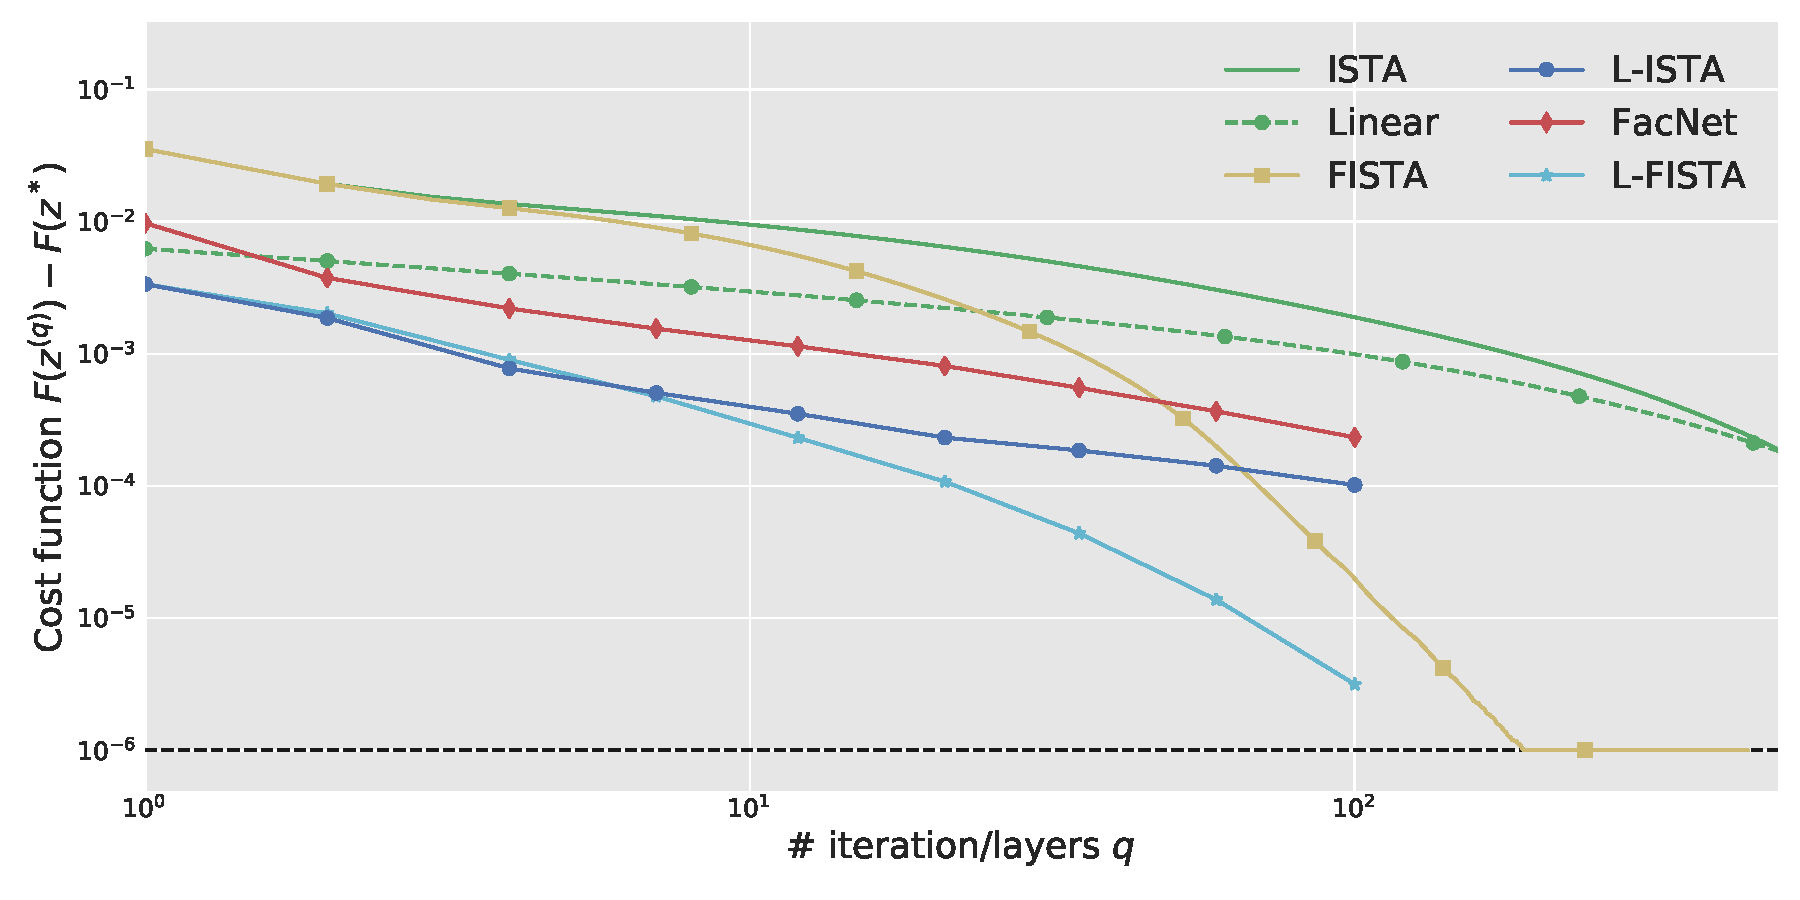
\includegraphics[width=\textwidth]{curve_images_seaborn}\\
     Evolution of the cost function $F(z^{(q)})-F(z^*)$ with the number of layers
     or the number of iteration $q$ for Pascal VOC 2008.
}
\end{frame}


\begin{frame}{MNIST}
\twocols{
	\btitle{MNIST}
	\vskip1em
	Dictionary $D$ with $K=100$ atoms learned on 10 000 MNIST samples (17x17) with dictionary learning.
	LISTA trained with MNIST training set and tested on MNIST test set.\\[1em]
}{
    \centering
    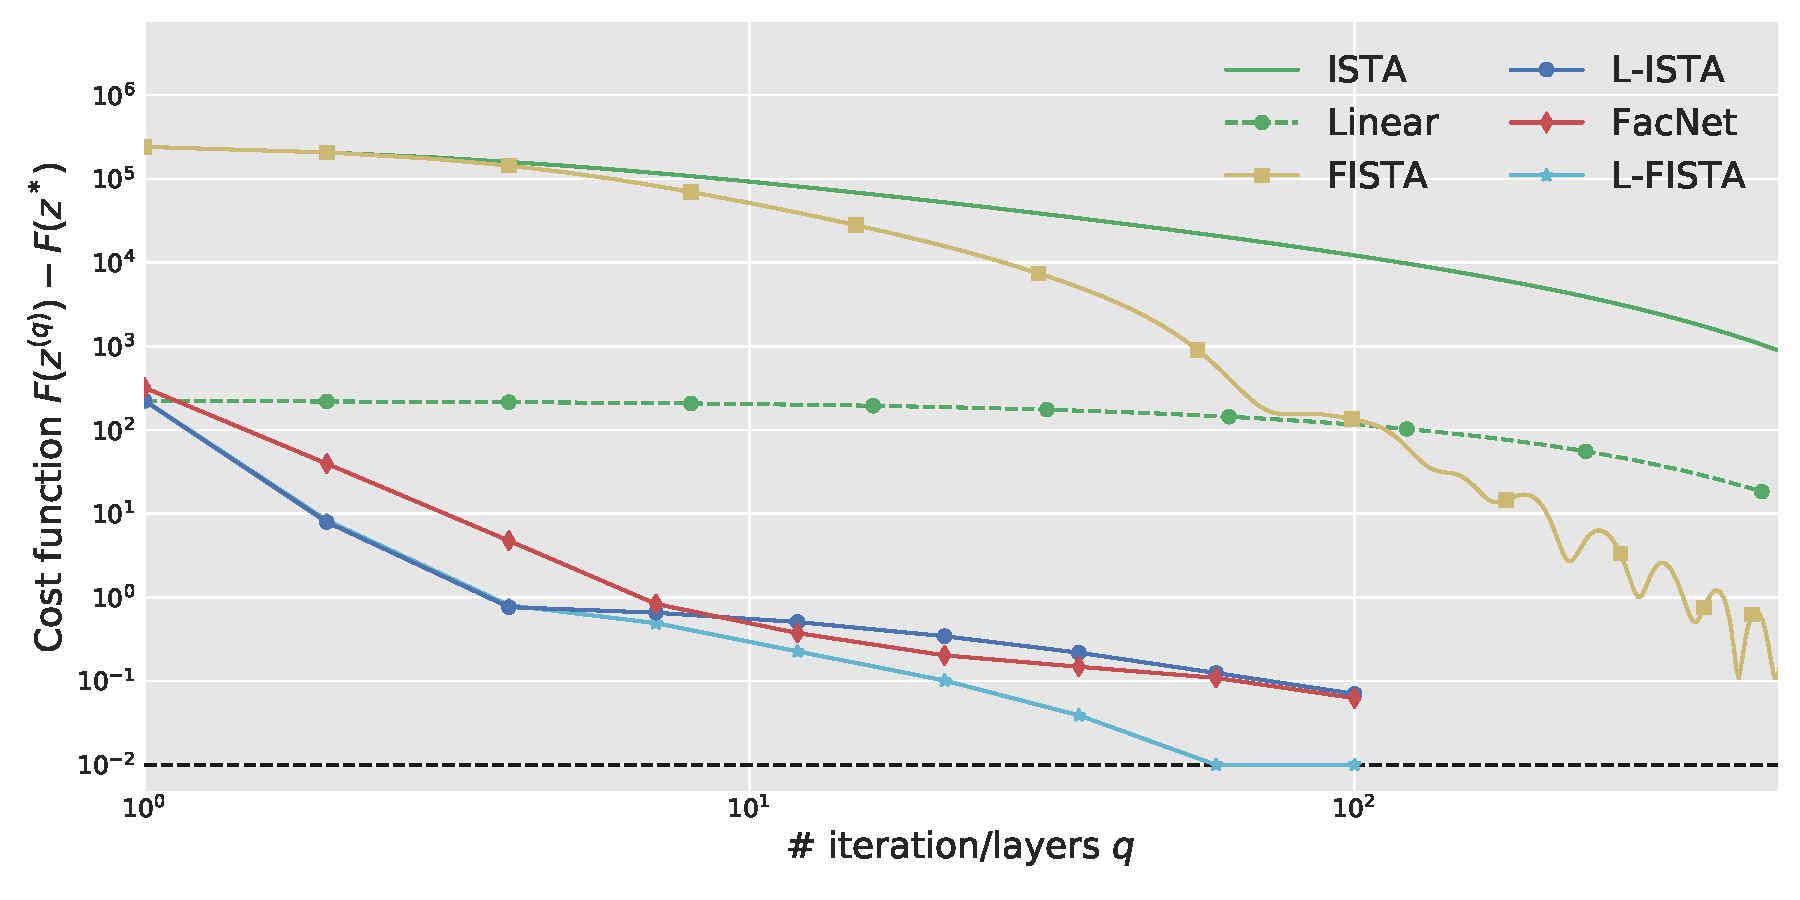
\includegraphics[width=\textwidth]{curve_mnist_seaborn}\\
     Evolution of the cost function $F(z^{(q)})-F(z^*)$ with the number
     of layers or the number of iteration $q$ for MNIST.
}{}
\end{frame}


%====================================================================
\subsection{DICOD}
%====================================================================

\begin{frame}{}

	\twocols{
	\btitle{Finishing the process in a linear grid?}
	Non trivial point: {\bf How to decide that the algorithm has converged?}\\[2em]
	
	\begin{itemize}\itemsep2em\itemindent1em
		\item Neighbors paused is not enough!
		\item Define a master 0 and send probes.\\
			\hskip3em Wait for $M$ probes return.
		\item Uses the notion of message queue and network flow.\\
			\hskip3emMaybe we can have better way?
	\end{itemize}
	}{}
	
	
\end{frame}

\begin{frame}
	\twocols{
		\centering
		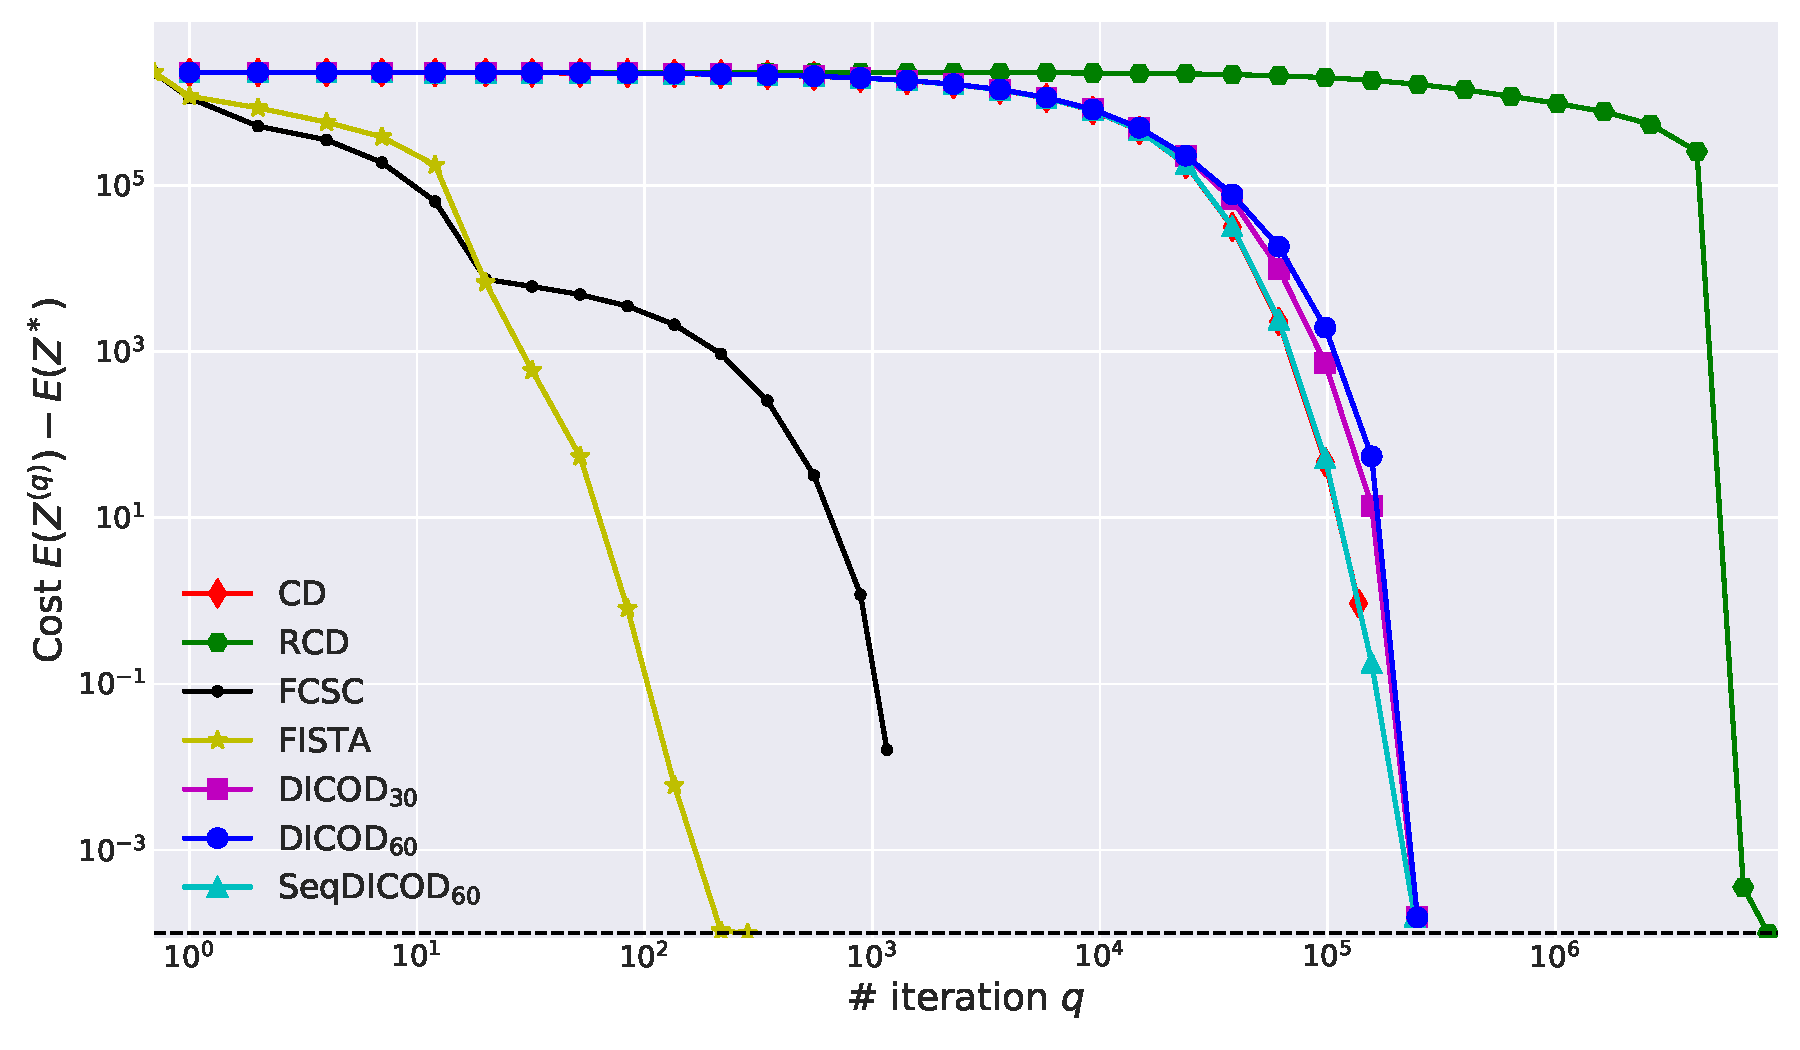
\includegraphics[width=\textwidth]{cost_seaborn_iter}\\
		\large Cost as a function of the iterations
	}{
		\centering
		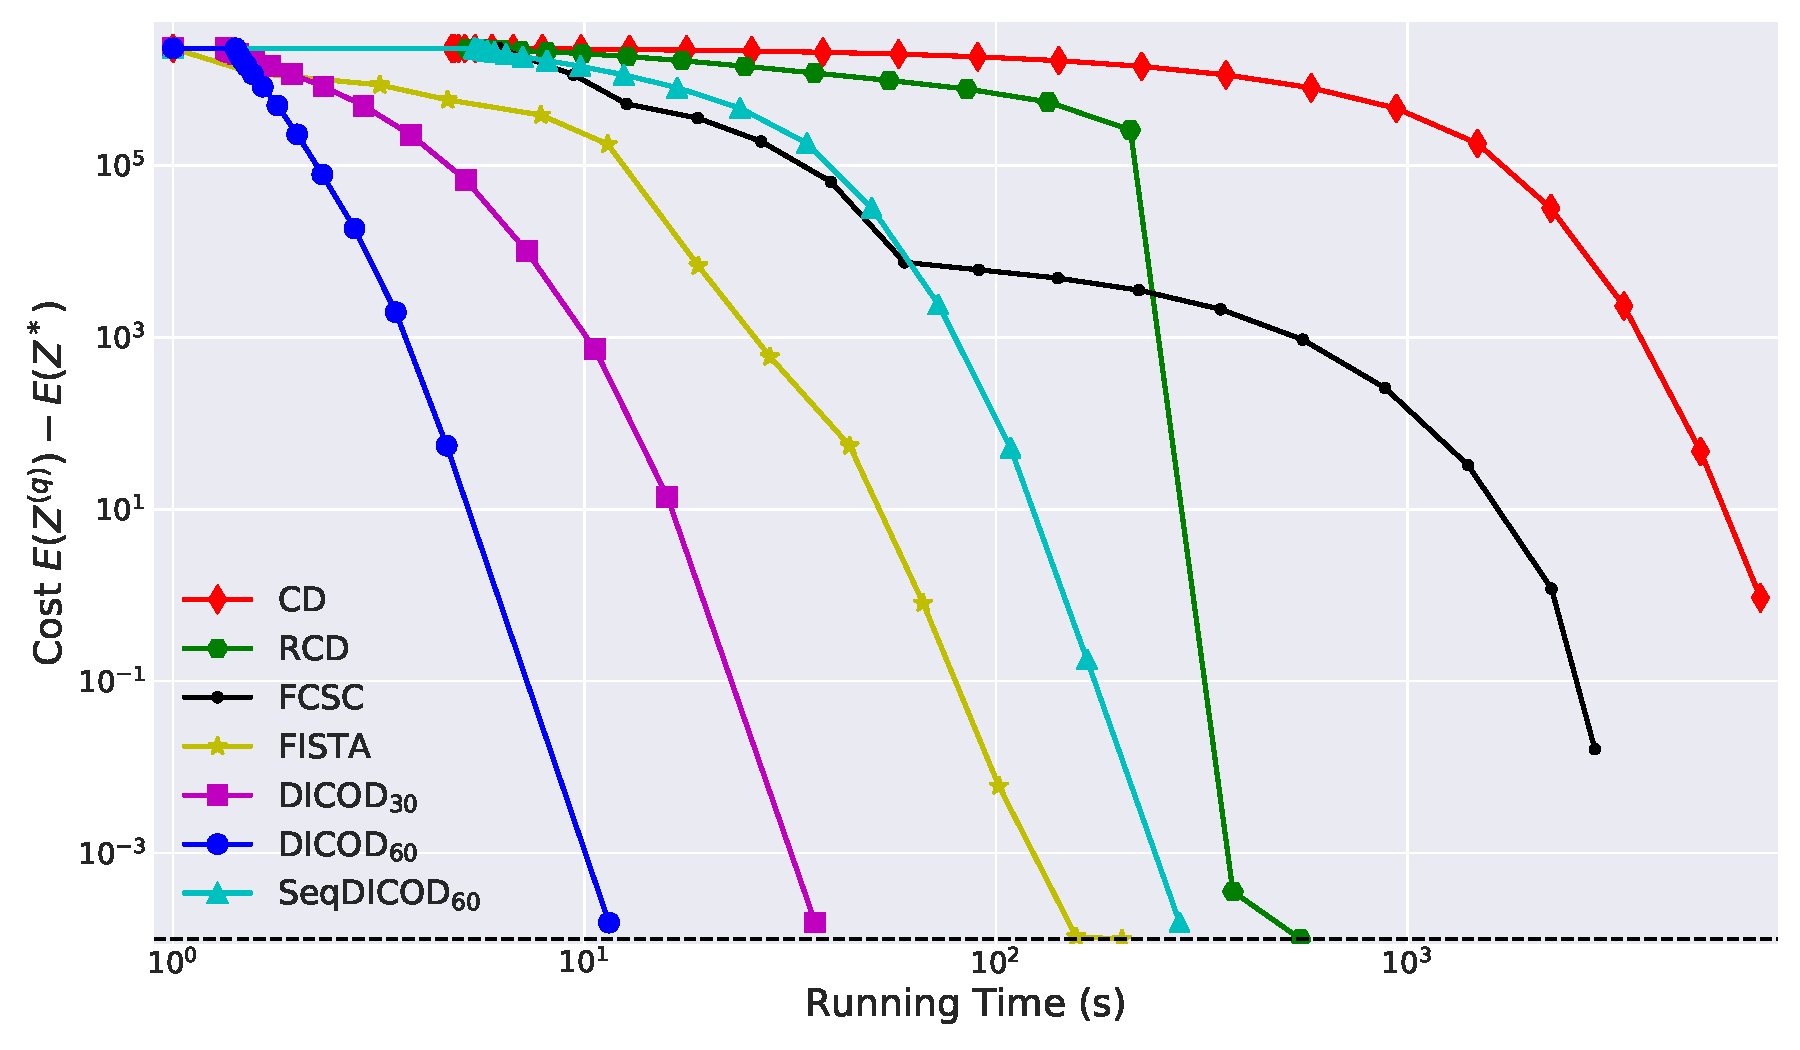
\includegraphics[width=\textwidth]{cost_seaborn_time}\\
		\large Cost as a function of the time
	}
\end{frame}



%====================================================================
\subsection{Singular Spectrum Analysis (SSA)}
%====================================================================

\begin{frame}{Singular Spectrum Analysis (SSA) \mycite{Vautard1989}}
	\twocols{
		\btitle{Sinuglar Spectrum Analysis}
		\vskip2em
		\begin{itemize}
			\item Choose a window size $K$ and extract sub series,
			\item Reconstruct a low rank estimate of all the $K$-length sub series,
			\item Decomposition of the series as a sum of "low rank" components.
		\end{itemize}
		}{
		{\usebeamercolor[bg]{itemize}.}\vskip2.5em
		\begin{itemize}\itemsep1em
		\item[$\rightarrow$] K-trajectory matrix $\pmb X^{(K)}$
		\item[$\rightarrow$] Singular Value decomposition
		$X^{(K)} = \sum_{k=1}^K \lambda_k U_kV_k^T$
		\item[$\rightarrow$] Average along anti-diagonals
	\end{itemize}
	}
	\vskip2em
	\bimplies{Extract components linked to trend and oscillations}
\end{frame}



\begin{frame}{Singular Spectrum Analysis}
\twocols{
	\vskip2em
	Linked to the convolutional least square
\begin{equation}\label{eq:sparse_code}
	Z^*, \pmb D^* = \arg\min_{Z, \pmb D} \frac{1}{2} \left\|X - \sum_{k=1}^K z_k*D_k\right\|_2^2,
\end{equation}
with constraints $\langle D_i, D_j \rangle = \delta_{i, j}$ 


\vskip1em
\begin{itemize}
	\item $\pmb D$ is the dictionary with $K = W$ patterns in $\mathbb R$ of length $W$
	\item $Z$ is an activation signal, or coding signal in $\mathbb R^K$ of length $L = T-W+1$
\end{itemize}
}{
	\vskip3em
	{\bf Issues}\\[1em]
	\begin{itemize}\itemsep1em\itemindent1em
	\item Same pattern present in different components,
	\item Representation is "dense", no localization,
	\item Different representation for each signal,
	\item A grouping step necessary to clean the extracted patterns.
	\end{itemize}
}
\end{frame}


\begin{frame}{Detrending with oculo}
	
\end{frame}



%====================================================================
\subsection{Post-training for Deep Learning}
%====================================================================


\begin{frame}{Post-training for Deep Learning}
\twocols{
	\btitle{Post-training}
	\vskip1em
	{\bf Paper with J. Audiffren: } arxiv:1611.04499\\[2em]

	Use the idea to split the representation learning and the task resolution:\\[1em]
	\begin{itemize}\itemindent1em\itemsep1.5em
		\item \underline{{\it Post-training} step:} only train the last layer,
		\item \underline{Easy problem:} this problem is often convex,
		\item \underline{Link with kernel:} close form solution for optimal last layer,
		\item \underline{Experiments:} consistent performance boost with multiple architecture.
	\end{itemize}
	}{
	\vskip3em
		{\bf Remarks}\\[1em]
	\begin{itemize}\itemsep1em\itemindent1em
	\item No gain if we are in a local minima,
	\item Should be use with early stopping.
	\end{itemize}
	}
	
\end{frame}



\end{document}
